\documentclass[varwidth, border =7pt]{standalone}
\usepackage{tikz}
\begin{document}

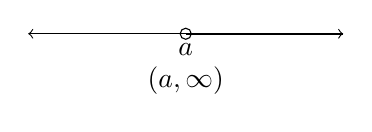
\begin{tikzpicture} %opið oendanlegt bil
\draw (2,0) circle (2pt) node[below] {$a$};
%\draw (3,0) circle (2pt) node[below] {$b$};
\draw[<->] (0,0) -- (4,0);
\draw[thick] (2,0) -- (4,0);
\node (c) at (2,-0.6) {$(a, \infty)$};
%\draw[thick] (0,0)--(3,0);
\end{tikzpicture}

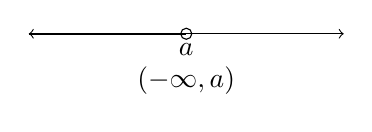
\begin{tikzpicture} %opið oendanlegt bil
\draw (2,0) circle (2pt) node[below] {$a$};
%\draw (3,0) circle (2pt) node[below] {$b$};
\draw [<->] (0,0) -- (4,0);
\node (c) at (2,-0.6) {$(-\infty,a)$};
\draw[thick] (0,0) -- (2,0);
%\draw[thick] (,0)--(3,0);
\end{tikzpicture}

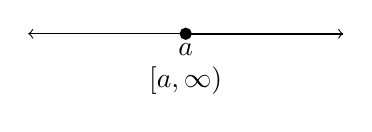
\begin{tikzpicture} %opið oendanlegt bil
\filldraw[black] (2,0) circle (2pt) node[below] {$a$};
%\draw (3,0) circle (2pt) node[below] {$b$};
\draw[<->] (0,0) -- (4,0);
\draw[thick] (2,0) -- (4,0);
\node (c) at (2,-0.6) {$[a, \infty)$};
%\draw[thick] (0,0)--(3,0);
\end{tikzpicture}

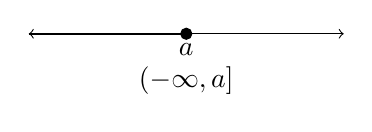
\begin{tikzpicture} %opið oendanlegt bil
\filldraw[black] (2,0) circle (2pt) node[below] {$a$};
%\draw (3,0) circle (2pt) node[below] {$b$};
\draw [<->] (0,0) -- (4,0);
\node (c) at (2,-0.6) {$(-\infty,a]$};
\draw[thick] (0,0) -- (2,0);
%\draw[thick] (,0)--(3,0);
\end{tikzpicture}

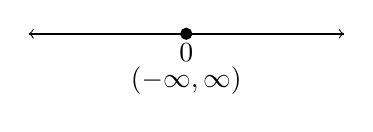
\begin{tikzpicture} %opið oendanlegt bil
\filldraw[black] (2,0) circle (2pt) node[below] {$0$};
%\draw (3,0) circle (2pt) node[below] {$b$};
\draw [<->] (0,0) -- (4,0);
\node (c) at (2,-0.6) {$(-\infty,\infty)$};
\draw[thick] (0,0) -- (4,0);
%\draw[thick] (,0)--(3,0);
\end{tikzpicture}

\end{document}
